\documentclass[output=paper]{langsci/langscibook}
\ChapterDOI{10.5281/zenodo.4280631}
\author{Hedde Zeijlstra\affiliation{Georg-August-Universität Göttingen}}
\title{Rethinking remerge: Merge, movement and music}

% \chapterDOI{} %will be filled in at production

%\epigram{Change epigram in chapters/03.tex or remove it there }

\abstract{In an influential paper, \citet{KatzPes2011} present the identity
    thesis for language and music, stating that \textquote{[a]ll formal
        differences between language and music are a consequence of differences
        in their fundamental building blocks (arbitrary pairings of sound and
        meaning in the case of language; pitch classes and pitch-class
    combinations in the case of music).  In all other respects, language and
music are identical.} \citeauthor{KatzPes2011} argue that, just like syntactic
structures, musical structures are generated by (binary) \isi{Merge}, for which they
provide a number of arguments: for instance, musical structures are endocentric
(each instance of \isi{Merge} in music, just like in language, has a labelling\is{labelling} head).
They also argue that \isi{movement} phenomena (i.e., the application of Internal
Merge) can be attested in both language and music. While fully endorsing the
view that musical structures are the result of multiple applications of
External (binary) \isi{Merge}, this paper argues that the arguments in favour of the
presence of Internal \isi{Merge} in music are at best inconclusive and arguably
incorrect. This is, however, not taken as an argument against the identity
thesis for language and music; rather, I take it to follow from it: the
identity thesis for language and music reduces all differences between language
and music to its basic building blocks. If the application of Internal \isi{Merge} in
natural language is driven by uninterpretable features
\parencite[cf.][]{Chomsky1995,Chomsky2001,Boskovic2007,Zeijlstra2012} that are
language-specific and not applicable to music (the reason being that only
building blocks that are pairings of sound and meaning can be made up of
interpretable and uninterpretable features), the direct consequence is that
Internal \isi{Merge} cannot be triggered in music either.}


\begin{document}\glsresetall\glsunset{EPP}
\maketitle

\section{Introduction: External and Internal Merge in language and
music}\label{sec:26.1}

Since \citet{Chomsky1995}, the operation \isi{Merge} has been taken to be the
primary structure-building operation in natural language. In current
minimalism, syntactic \isi{movement} is, moreover, considered a special instance of
Merge (Internal Merge), which applies to a particular syntactic object and a
part thereof (cf., inter alia, \citealt{Chomsky2005}). In this sense, Internal
Merge is different from External \isi{Merge}, where the two input objects do
not stand in an inclusion relation.

However, natural language is not the only cognitive domain where \isi{Merge} is
said to be a structure-building operation. As has been claimed in
\citet{LerJac1983} and, more recently, in \citet{KatzPes2011}, music is also a
cognitive domain where structures can be taken to be generated by means of an
operation like \isi{Merge}. If musical structures are indeed generated by means
of \isi{Merge} and if \isi{movement} is a special instance of \isi{Merge}, the
question arises whether music exhibits \isi{movement} effects as well. After all, why
could Internal \isi{Merge} not apply in music if it can apply in natural
language?

In order to account for the differences and similarities between language and
music, \citet{KatzPes2011} entertain their so-called \emph{identity thesis for
language and music}\is{identity thesis for language and music}, which states
that:

\blockquote[{\citealt[3]{KatzPes2011}}][.]{[a]ll formal differences
    between language and music are a consequence of differences in their
    fundamental building blocks (arbitrary pairings of sound and meaning in the
    case of language; pitch-classes and pitch class combinations in the case of
music). In all other   respects, language and music are identical}

For \citeauthor{KatzPes2011}, this means that \isi{Merge} should be equally
effective in natural language and music and that therefore music is indeed
expected to exhibit both External and Internal \isi{Merge} effects. In their
paper, they identify particular musical patterns that they take to reflect
movement in music.

However, one may wonder whether it is correct to assume that \isi{identity
thesis for language and music} entails that both External and Internal
\isi{Merge} should apply in music. As I will argue in this paper, it all
depends on what triggers Internal \isi{Merge} in the first place. Internal
\isi{Merge} differs from External \isi{Merge} in the sense that Internal \isi{Merge}
does not have to take elements from the numeration into the syntactic
structure. If every element in the numeration needs to end up in the syntactic
structure, it follows immediately that every element present in the numeration
needs to undergo External \isi{Merge}. But why would particular elements be
required to undergo Internal \isi{Merge} as well?

Following a longstanding tradition in syntactic theory, I assume that Internal
Merge is triggered by so-called uninterpretable formal features -- formal
features that need to stand in a particular configuration with their
interpretable counterparts. If that is the case, the question arises as to
whether such movement-triggering features can also be attested in music. I
argue they do not.

According to the \isi{identity thesis for language and music}, all differences
between music and language should reduce to differences in their building
blocks: for \citeauthor{KatzPes2011}, arbitrary pairings of sound and meaning
in the case of language, and pitch classes and pitch-class combinations in the
case of music. Let’s focus in more detail on each type of building blocks.

Lexical items are generally thought to consist of three types of features:
phonological features, syntactic or formal features, and semantic features.
Phonological features are only interpretable or legible for the sensori-motor
system; semantic features are only interpretable or legible for the
conceptual-intentional systems; and syntactic or formal features are
interpretable or legible for neither of them. In that sense, linguistic
building blocks can be said to be multi-modular, not mono-modular.

Things are different when it comes to musical building blocks. One dimension in
which the architecture of music is much different from that of natural language
is that musical structures are not subject to compositional semantic
interpretation in the sense that the meaning of a musical structure – to the
extent it has any (see, for instance, \citealt{Schlenker2016} and references
therein for discussion)~– follows compositionally from the meaning of the parts
it consists of and the way these parts are structured. While linguistic objects
are built of elements that form sound-meaning pairs, the musical objects are
not. Musical building blocks are mono-modular building blocks. Mono-modular
building blocks are building blocks that are all interpretable or legible for
the same module, in this case the sound side of music. And even if it turns out
that pitch classes and pitch-class combinations are not the only available
building blocks in music (and other building blocks are available as well,
either inside or outside Western tonal music), those building blocks will still
belong to the same sound module.

Mono- vs.\ multi-modularity is then a main characteristic of the differences
between musical and linguistic building blocks. Now, under the view that the
application of Internal \isi{Merge} is indeed driven by the need of so-called
uninterpretable features to be checked by their interpretable counterparts, it
follows immediately that Internal \isi{Merge} can only be triggered by features
present on linguistic building blocks, not on musical building blocks. The
reason is that uninterpretable features are defined as elements that are not
part of the set of semantic features, but require a particular checking (or
valuation) relation with a feature that does belong to this set. As a
consequence, no uninterpretable feature can be acquired without the presence of
a semantic counterpart
\parencite[see][]{Brody1997,Svenonius2007,Zeijlstra2008,Zeijlstra2012}. But if
that is correct, uninterpretable features, by definition, can only be part of
building blocks that are not mono-modular. In fact, in any cognitive system
whose output is not defined in terms of pairs of elements belonging to
different cognitive modules (in the way that linguistic output is defined in
terms of sound-meaning pairs), features that denote dependencies on elements
belonging to different modules cannot exist.

If that is the case, the \isi{identity thesis for language and music} should
actually predict that, to the extent that Internal \isi{Merge} can only be
triggered by uninterpretable formal features, it can never apply to pieces of
musical structure and that therefore instances of \isi{movement} are expected to be
absent in music.

In this article, I first further elaborate the claim that (properties of)
uninterpretable features are the trigger for syntactic \isi{movement}
(\sectref{sec:26.2}). Then, in \sectref{sec:26.3}, I discuss Katz \&
Pesetsky’s claim that music does not only exhibit External \isi{Merge}, but
also Internal \isi{Merge}. In \sectref{sec:26.4}, I spell out some problems
for the claim that music exhibits \isi{movement} effects, and I provide an
alternative analysis for the phenomena discussed by \citeauthor{KatzPes2011}
that does not allude to \isi{movement}. I argue that this alternative account can
equally well, if not better, explain the special behaviour of full cadences
than the \isi{movement} account does.  \sectref{sec:26.5} concludes.

\section{Internal and External Merge in natural language}\label{sec:26.2}

One of the highlights of the twenty-first-century developments in minimalism
has been the operational unification of syntactic structure building and
movement. While previous versions of minimalism (and its generative
predecessors) took \isi{movement} to involve a separate syntactic operation alongside
Merge (or any other structure-building operation), \citet{Chomsky2005} argued
that nothing a priori forbids \isi{Merge} to apply to previously created parts
of the syntactic structure, and to remerge, or internally merge, these with the
top node of the derivation (see also \citealt{Starke2001}). Under this
conception of Internal \isi{Merge}, the question as to why natural language
would display displacement operations no longer seemed to be in need of an
explanation. If \isi{Merge} is not restricted to External \isi{Merge}, it would
rather require additional explanation if language did not display \isi{movement}
effects.

At the same time, questions still arise with respect to when Internal \isi{Merge}
should take place. Internal \isi{Merge} differs from External \isi{Merge} in
the sense that Internal \isi{Merge} does not have to take elements from the
numeration into the syntactic structure. If every element in the numeration
needs to end up in the syntactic structure, it follows immediately that every
element present in the numeration needs to undergo External \isi{Merge}. But
why would particular elements be required to undergo Internal \isi{Merge} as
well? From this perspective, there is no (external) reason that would force
Internal \isi{Merge} to take place.

The most straightforward solution would be to assume that Internal \isi{Merge}
only takes place if not applying it would render the sentence ungrammatical.
Under that view, Internal \isi{Merge} is a costly operation that only applies
when necessary. This means that it is an operation for which a trigger is
needed; and therefore, the question immediately arises as to what triggers
Internal \isi{Merge}.

Originally, it has been proposed by \citet{Chomsky1995} that so-called
uninterpretable features trigger \isi{movement}. In a structure like
(\ref{ex:26.1}), it is the uninterpretable [u${\varphi}$] feature on T that
triggers \isi{movement} of the lower DP into the specifier position of the T-head, so
that this feature, as well as the nominative\is{nominative case} feature on the DP, can be checked.
The central conceptual motivation behind uninterpretable features as triggers
for \isi{movement} was that this would reduce two not well understood phenomena
– the existence of semantically vacuous elements and the existence of
displacement effects – to one not well understood notion: the need to remove
uninterpretable features (where removal of uninterpretable features was said to
take place under spec-head configuration).

\ea\label{ex:26.1}
    \begin{tikzpicture}[baseline]

        \Tree 	[.TP
                    \node (dp) {DP\tss{[\sout{\Nom}][φ]}};
                    [.T$'$
                        T\tss{[finite][\sout{uφ}]}
                        [.vP
                            \node (t) {DP\tss{[\Nom][φ]}};
                            \dots{}
                        ]
                    ]
                ]

        \draw [->] (t) -- +(0,-.5) -| (dp);

    \end{tikzpicture}
\z

This view, however, was later on rejected, primarily since it turned out that
uninterpretable features could be checked at a distance (the uninterpretable
feature probing down in its c-command domain to find a matching active goal).
English expletive\is{expletives} constructions (where the finite verb agrees with a lower
VP-internal associated subject) \REF{ex:26.2}, \ili{Icelandic} quirky case
constructions (where the verb agrees in number with a nominative\is{nominative case} object)
\REF{ex:26.3}, and various other constructions all underlie structures
where the probe and the goal of \isi{agreement} never appear in spec-head
configuration:

\ea\label{ex:26.2}
    \ea There seems to have arrived some student.
    \ex There seem to have arrived some students.
    \z
\ex\label{ex:26.3} \ili{Icelandic} \parencite{Bobaljik2008} % Saint-Etienne?
    \ea
    \gll    Jóni líkuđu thessir sokkar\\
            Jon.\textsc{dat} like.\textsc{pl} these socks.\textsc{nom}\\
    \glt    \enquote*{Jon likes these socks.}
    \ex
    \gll    Mér virdast hestarnir vera seinir\\
            me seem. \textsc{pl} the.horses be slow\\
    \glt    \enquote*{It seems to me that the horses are slow.}\\
    \z
\z

If uninterpretable features can no longer be taken to trigger Internal
\isi{Merge}, the question arises as to what should do instead.
\textcite{Chomsky2000,Chomsky2001} argues that \isi{movement} should be thought of as
an operation dependent on, and not triggered by, \isi{agreement}. For him, probes,
carrying uninterpretable features, could be equipped with an additional feature
[EPP],\is{extended projection principle} which requires that the specifier of the probing head be filled. If no
other suitable candidate could be merged externally in that position (such as
an expletive\is{expletives} subject like English \emph{there}, or a dative\is{dative case} subject, to the
extent that such elements could be externally merged in this position in the
first place; cf.\ \citealt{Chomsky2000,Deal2009} for different proposals and
discussion), the goal would raise into that position.

Even though using the \gls{EPP}-feature \is{extended projection principle}gets
these facts right, its postulation has often been criticized for a lack of
independent motivation. The \gls{EPP}-feature \is{extended projection
principle}is rather a movement-triggering diacritic and does not build upon any
explanation as to why \isi{movement} should take place in the first place,
although it could be that the presence or absence of \isi{movement}
(diacritics) is really just formal arbitrariness (a position taken by
\citealt{BibHolRob2009,BibHolRobShee2014,BibRob2015}, among others).  For this
reason, others have proposed to reinstall uninterpretable features themselves,
rather than \gls{EPP}-features\is{extended projection principle}, to be the
sole triggers of \isi{movement} (e.g.,~\citealt{BjoZei2019}). Nevertheless,
whether uninterpretable features or subfeatures of uninterpretable features are
the trigger for \isi{movement}, in both cases uninterpretable features still
form necessary elements in movement-triggering configurations.

Naturally, it is not the case that \gls{EPP}-features\is{extended projection principle} and (un-)interpretable features are the only candidates for being
movement triggers. \citet{Richards2016}, for instance, has argued that
phonological adjacency requirements trigger \isi{movement}; and \citet{NeeKoo2008}
have argued that \isi{movement} may feed various mapping rules. But it should be
noted that this type of approaches also relates the necessity of \isi{movement} to
interface requirements, as do uninterpretable feature approaches. This all
suggests that, in cognitive systems that lack formal features mediating between
phonological and semantic features, triggering of Internal \isi{Merge} might
not be possible.

\section{Internal and External Merge in music}\label{sec:26.3}

In this section, I discuss the extent to which \isi{Merge} can be said to be
the (sole) structure-building operation in music, as claimed by
\citeauthor{KatzPes2011}.  In order to provide evidence for this claim,
\citeauthor{KatzPes2011} build upon the insights presented in
\citegen{LerJac1983} \glsunset{GTTM}\emph{\glsdesc{GTTM}} (\gls{GTTM}). I will
first briefly illustrate the major components of \gls{GTTM}\is{Generative
theory of tonal music} that are relevant for the discussion in this paper,
without doing justice to the richness of this theoretical framework
(\sectref{sec:26.3.1}). Then, in \sectref{sec:26.3.2}, I will present a
particular aspect of music, namely the existence of structural hierarchies in
music, which, for \citeauthor{KatzPes2011}, forms evidence for their claim that
musical structures are generated by at least External \isi{Merge}.  In
\sectref{sec:26.3.3}, I discuss how, according to \citeauthor{KatzPes2011},
other musical properties provide evidence for Internal \isi{Merge} in music.

\subsection{Lerdahl \& Jackendoff’s Generative theory of tonal music}
\label{sec:26.3.1}

According to the \gls{GTTM}\is{Generative theory of tonal music} model, there
are four components that determine the proper analysis of a musical structure.
These four components are listed/given in \REF{ex:26.4} below:

\ea\label{ex:26.4}
    \ea grouping structure
    \ex metrical structure
    \ex \gls{TSR}
    \ex \gls{PR}
    \z
\z

Following \textcite[8--9]{LerJac1983}, grouping structure “expresses the
hierarchical segmentation of the piece into motives, phrases, and sections”;
metrical structure “expresses the intuition that the events of the piece are
related to a regular alternation of strong and weak beats at a number of
hierarchical levels”; \gls{TSR} “assigns to the pitches of the piece a
hierarchy of \enquote{structural importance} with respect to their position in
grouping and metrical structure”; and \gls{PR}, finally, “assigns to the
pitches a hierarchy that expresses harmonic and melodic tension and relaxation,
continuity and progression”.

For \citet{LerJac1983}, each component can assign a set of structures to a
given string of music; and an additional set of preference interface rules then
determines which of these analyses is the correct one (often just one). In this
sense, the musical architecture forms a strong resemblance with Jackendoff’s
parallel architecture of grammar
(\citealt{Jackendoff1997,Jackendoff2002,CulJac2005}), which treats phonology,
syntax, and semantics as independent generative components whose structures are
also linked by interface rules: each component generates (a number of)
structures, and interface rules determine what the proper mappings between
these structures are. Such interface rules, for instance, determine which
prosodic and which syntactic structures correlate.

Jackendoff’s parallel architecture differs from Minimalist grammar in the sense
that parallel architecture grammar has multiple engines, whereas Minimalist
grammar has only one engine: its output leading to different levels of
representation (\gls{PF} and \gls{LF}). However, at least according to
\citeauthor{KatzPes2011}, and I follow them in this respect, it is not the case
that every musical component may bi-directionally inform every other component.
Rather, it turns out that the outputs of grouping structure and metrical
structure both inform \gls{TSR}, which, in turn, informs \gls{PR}. But if that
is the case, the model for a grammar of music can be thought of as these
components being directionally ordered, much like different grammatical
components are directionally ordered in Minimalist grammar (\figref{fig:26.6}).
\citeauthor{KatzPes2011}’s implementation of GTTM (\figref{bkm:Ref348624990}) is
the reverse of the reverse Y-model.

\begin{figure}
\begin{floatrow}
  \captionsetup{margin=.05\linewidth}
  \ffigbox{%
    \begin{tikzpicture}[baseline, node distance=1cm and 1cm]
        \node (tsr) {\glsdesc{TSR}};
        \node [align=center,above left = of tsr.north] (gs) {grouping\\structure};
        \node [align=center,above right = of tsr.north] (ms) {metrical\\structure};
        \node [below = of tsr] (pr) {\glsdesc{PR}};
        \draw [->, shorten <=.5mm, shorten >=.5mm] (gs.south) to (tsr.north);
        \draw [->, shorten <=.5mm, shorten >=.5mm] (ms.south) to (tsr.north);
        \draw [->, shorten <=.5mm, shorten >=.5mm] (tsr.south) to (pr.north);
    \end{tikzpicture}%
    }
    {\caption{\label{bkm:Ref348624990}\citegen{KatzPes2011} (reverse reverse) Y-model of the grammar of music}}
  \ffigbox{%
    \begin{tikzpicture}[baseline, node distance=1cm and 1cm]
        \node (sx) {syntax};
        \node [below left = of sx.south] (pf) {phonology};
        \node [below right = of sx.south] (lf) {semantics};
        \node [above = of sx] (lex) {lexicon};
        \draw [->, shorten >=.5mm] (sx.south) to (lf.north);
        \draw [->, shorten >=.5mm] (sx.south) to (pf.north);
        \draw [->, shorten <=.5mm, shorten >=.5mm] (lex.south) to (sx.north);
    \end{tikzpicture}%
    }
    {\caption{\label{fig:26.6} The reverse Y-model of the grammar of natural language}}
\end{floatrow}
\end{figure}

If this implementation is correct, the architecture of musical grammar forms a
striking correspondence with the architecture of natural language grammar. A
particular input is assigned an initial structure that can be derivationally
transformed in subsequent structures, with particular well-formedness
conditions\linebreak holding at different levels of representation.

Under this architecture, it can indeed be investigated what the exact parallels
are between the syntax of music and the syntax of natural language, and, most
notably, whether the differences attested between language and music are merely
a consequence of the differences in their building blocks or whether these
differences are richer in nature.

\subsection{External \isi{Merge} in music}\label{sec:26.3.2}

For \citeauthor{LerJac1983} and for \citeauthor{KatzPes2011}, the
correspondence between language and music is stronger than merely being an
architecture with various components that together are responsible for the
analysis of a structure (irrespective of whether these components are
derivationally or representationally connected by means of interface rules). As
\citeauthor{LerJac1983} already proposed, \gls{TSR} in \gls{GTTM}\is{Generative
theory of tonal music} is very similar to prosodic structure in natural
language, as both are formulated in terms of relative prominence. Moreover,
\citeauthor{KatzPes2011} take \gls{PR} to align with linguistic syntax.  The
reason for them is that both \gls{PR} and linguistic syntactic structures are
binary branching, endocentric (i.e., headed) structures of the kind that is
created by (External) \isi{Merge} in Minimalist grammar. That such structures
are headed can be witnessed by the fact that such structures are able to encode
dependency relations between non-string-adjacent elements.

To see this, let us focus on the structure of \gls{PR}. \gls{PR} structures
assign to the pitches a hierarchy that expresses harmonic and melodic tension
and relaxation, continuity and progression. Simplifying things, every pitch
that increases some kind of tension needs to be followed by some kind of
relaxation. However, this need for tension followed up by relaxation is
crucially not a string-adjacent condition. In fact, as we will see later on, it
may very well be the case that the first tonic already induces a tension that
is to be relieved by the final tonic, thus creating a constituent of two
sisters whose heads span the entire musical piece. That means that tensions and
relaxations in musical structures form non-local dependencies that are best
explained as structural dependencies.  This intuition is encoded in \glspl{PR}
by assigning head status to any sister of a node that is more relaxed.
As an example, take the toy melody in \figref{bkm:Ref348696475}.

\begin{figure}
\caption{\label{bkm:Ref348696475}Toy melody
\parencite[16]{KatzPes2011}}
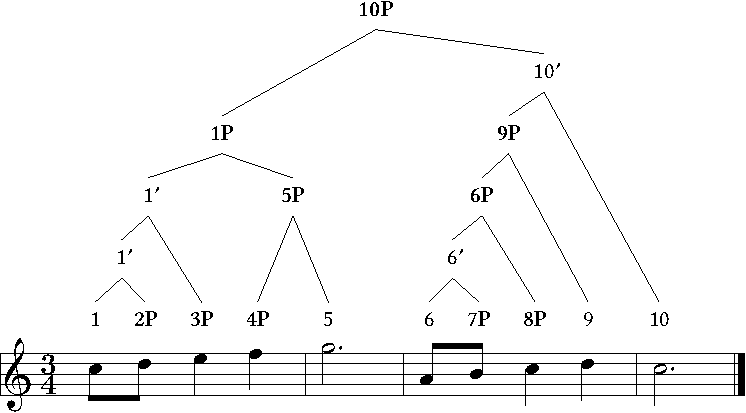
\includegraphics[width=\textwidth]{./img/28-7.pdf}
\end{figure}

In this structure, the first event (the tonic C) establishes a sisterhood
relation with the second event, the tonic being the head. In Western tonal
music, tonics are always the most relaxed pitches, whereas pitches or chords
based on pitches belonging to other scale degrees are felt to be tenser.
Accordingly, the first event in this toy melody is the head of the merger with
the second, third, fourth, and fifth events. The fifth event is the dominant
(five degrees away from the tonic), which is tensed with respect to the tonic,
but more relaxed with respect to the so-called subdominant (here, the fourth
event), which is four degrees away from the tonic. Similarly, the final pitch
(again, a tonic C) creates similar dependencies with the sixth till ninth
events. The overall structure then consists of a constituent of two phrases:
one in which the tonic in the first event is the head (1P) and one in which the
tonic in the tenth event is the head (10P).

Evidence for this procedure of structure assignments comes from so-called
\emph{Schenkerian reductions} (see \citealt{Forte1959}). Schenkerian reductions
are best understood as musical summaries. Going bottom-up, removing every layer
of non-heads will still yield a melody that feels like the same kind of melody
as the intact structure. This process can in principle be continued until the
most prominent chords are left. By contrast, if an event with higher prominence
is left out, the piece is no longer perceived as a proper reduction. Examples,
taken again from \citet{KatzPes2011}, are presented below:\largerpage

\ea\label{ex:26.8}Good reductions of \figref{bkm:Ref348696475}
    \ea Deleting the non-heads of the lower 1$'$ and of 6$'$
        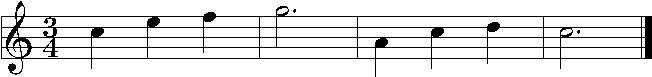
\includegraphics[scale=.9]{./img/28-8a.pdf}
    \ex Deleting the non-heads of the higher 1$'$ and of 6P
        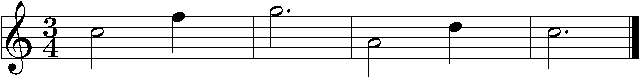
\includegraphics[scale=.9]{./img/28-8b.pdf}
    \ex Deleting the non-heads of the higher 1$'$, 5P and 9P
        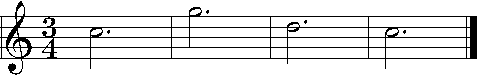
\includegraphics[scale=.9]{./img/28-8c.pdf}
    \z
\ex\label{ex:26.9}A bad reduction of
\figref{bkm:Ref348696475}\\[.66\baselineskip]
    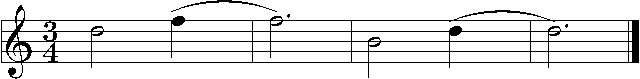
\includegraphics[scale=.9]{./img/28-9.pdf}
\z

What does this tell us about \isi{Merge} in music? The crucial comparison is
that the structure-building operation appears to be similar to (External)
\isi{Merge}. Every two musical objects (being atomic or non-atomic) may merge
and form a constituent of which the label is the same as that of one of its two
daughters (the head). But if that is correct, it can be seen as evidence for
there being a \enquote{syntactic engine} that is equally active in language and in
music. This would, of course, be fully in line with \citeauthor{KatzPes2011}’s
\isi{identity thesis for language and music}. It is the module-specific
properties of music that determine what elements can be merged and, once
merged, which ones yield the heads (in terms of tension and relaxation, to be
computed on the basis of scalar distance with respect to the tonic). But the
combinatorial mechanism, \isi{Merge}, applies to musical objects in exactly the same
way as it applies to syntactic objects.

\subsection{Internal \isi{Merge} in music}\label{sec:26.3.3}

The previous discussion of External \isi{Merge} in music sets the ground for
the next step in the discussion. If musical structures are indeed built by
means of the single generative operation \isi{Merge} (and the evidence for that
claim, confirming the \isi{identity thesis for language and music}, seems quite
strong), then the question arises as to whether only External \isi{Merge}
applies or whether Internal \isi{Merge} may apply as well. Formally, there is nothing
in the combinatorial procedure that would exclude Internal \isi{Merge} applying
to music. \citeauthor{KatzPes2011} argue that \isi{movement} effects can indeed
be attested in music. Let us first look at the arguments they present for that.

In order to assess whether musical pieces may display \isi{movement} effects, one
should first determine what the proper characteristics of \isi{movement} in music
would be. That task is far from trivial, as general diagnostics for \isi{movement}
(the surface position of some element does not correspond with the locus of its
semantic interpretation) do not apply in music, for the simple reason that
musical structures lack semantic interpretation (in the sense that musical
structures lack~\gls{LF}). Therefore, the diagnostics for \isi{movement} should
either be formal or PF-like. Moreover, such diagnostics are arguably different
for phrasal \isi{movement} and for \isi{head movement}. Since \citeauthor{KatzPes2011} do
not provide any evidence for the existence of phrasal \isi{movement} in music (even
though they explicitly do not rule it out per se), but rather focus on head
movement only, I will also only discuss what the characteristics of head
movement in music would be. The characteristics that \citeauthor{KatzPes2011}
apply for \isi{head movement} in language and music are given in \REF{ex:26.10}
and \REF{ex:26.11}, respectively:

\ea\label{ex:26.10}Head-movement in language \parencite[40]{KatzPes2011}
    \ea Once the head H of a phrase HP has undergone \isi{head movement}, H is
    pronounced string-adjacent to the head of a higher phrase, but at the same
    time \dots{}
    \ex \dots{} the rest of HP remains an independent phrase that behaves just
    like a phrase whose head has not moved -- even though:
    \ex The \isi{movement} is obligatory. Movement of finite V to T in \ili{French}
    satisfies some need of an element in this structure [\dots{}].
    \ex The zero-level head that undergoes \isi{head movement} to another zero-level
    head ends up tightly coupled to its new host. The two heads end up behaving
    like a single morphologically complex word for later processes of grammar
    (both syntactic and phonological).
    \z
\ex\label{ex:26.11}Head-movement in music \parencite[41]{KatzPes2011}
    \ea Some chord X must be performed string-adjacent to a chord Y. But at the
    same time \dots{}
    \ex \dots{} X has a normal set of syntactic dependents of its own,
    linearized normally -- and thus apparently also heads its own phrase (an
    XP);
    \ex The \isi{movement} should be obligatory, insofar as it produces an alteration
    in the features of Y that is required in order for the derivation to
    succeed;
    \ex Even though X may take a normal set of syntactic dependents, X is
    tightly coupled to its host Y, such that they function as an indivisible
    unit for other purposes (cf.\ the notion word).
    \z
\z

Here, I will not contest these characteristics for \isi{movement}, although I would
like to point out that these characteristics should be interpreted in a
uni-di\-rec\-tion\-al way. They are not diagnostics. Even if all effects attributed
to \isi{head movement} are indeed attested, this does not entail that the reverse
must be the case as well. If some ${\alpha}$ and ${\beta}$ are both heads,
pronounced string-adjacently, with ${\alpha}$ altering some feature of
${\beta}$ and ${\alpha}$ and ${\beta}$ together taken to form an indivisible
unit (i.e., behaving word-like), this does not necessarily entail that
${\alpha}$ underwent \isi{head movement} into ${\beta}$. I will come back to that in
\sectref{sec:26.4}.

\citeauthor{KatzPes2011} continue their argument by showing that so-called full
cadences are a musical phenomenon that shows all the characteristics of head
movement. In full cadences, the final chord, the tonic, which determines the
key and counts as the head of the entire musical structure, must be preceded by
a dominant, a chord whose root is five scale-steps away from the tonic and
which has at least one dependent, generally headed by the so-called
subdominant, often four scale-steps away from the tonic. In \gls{PR}, the
dominant is directly subordinate to the tonic and occupies a highly prominent
position; metrically, it is often felt to be a much weaker chord that seems
more deeply embedded in \gls{PR} and seems to act as a weaker dependent of the
tonic. This latter phenomenon is generally referred to as \emph{cadential
retention} – the phenomenon that the dominant and the tonic behave almost like
a joint chord (and are even analysed as such in GTTM). An example is provided
in \figref{bkm:Ref348897627}, where the dotted arrow (for now) indicates
the stronger dependency of the dominant (δ) on the tonic (τ) (ν indicating the
subdominant).

\begin{figure}
    \caption{\label{bkm:Ref348897627}Example of a full cadence \parencite[44]{KatzPes2011}}
    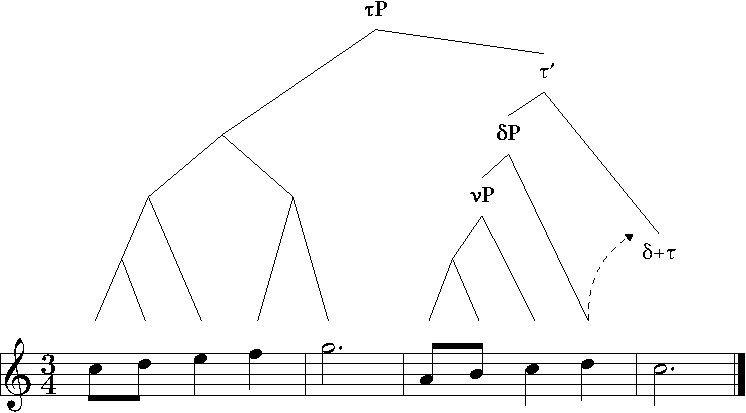
\includegraphics[width=\textwidth]{./img/28-12.pdf}
\end{figure}

Looking at the characteristics of \isi{head movement} in music,
\citeauthor{KatzPes2011} conclude that full cadences indeed are the result of
head \isi{movement}, and, therefore, of the application of Internal \isi{Merge} in
music.

As for the first two characteristics, if the dominant indeed raises into the
head position of the tonic (yielding the structure in (\ref{bkm:Ref348711137}),
where angled brackets indicate lower copies of moved elements), the dominant is
expressed string-adjacently to the tonic, even though the dominant still heads
a phrase of its own (δP). This way, the construction behaves exactly like the
first two clauses of the list of characteristics for \isi{head movement} (in music).

\ea\label{bkm:Ref348711137}
    {}[\tss{τP} [\tss{δP} [\tss{νP} ν \dots{} ] \tuple{δ} ] δ–τ]
\z

As for the third characteristic, \citeauthor{KatzPes2011} claim that \isi{movement}
of the dominant into the tonic marks the tonic for establishing the key of the
entire musical piece. They suggest that, in full cadences, \isi{movement} of the
dominant into the tonic head has the function of tonic-marking τ, i.e.,
assigning it the feature [$+$TON]. When the tonic head in a structure is
tonic-marked, the terminal nodes of the phrase headed by the tonic are
understood to belong to the key of τ. In this sense, head-movement of the
dominant alters the tonic in having the feature [$+$TON].

As for the fourth characteristic, finally, \citeauthor{KatzPes2011} argue that
moving the dominant into the tonic position makes the joint dominant–tonic
complex act more like a single unit in terms of metric position and makes the
dominant look structurally less important than its \gls{PR} position would
legitimize. This joint behaviour, then, is what underlies the phenomenon of
cadential retention.

On the basis of this analysis, \citeauthor{KatzPes2011} conclude that musical
structures are indeed generated by means of \isi{Merge}, and the fact that
Merge comprises both External and Internal \isi{Merge} predicts that musical
structures may indeed exhibit \isi{movement} effects, of which full cadences are then
an example.  And, if musical structures indeed allow for \isi{movement}, this forms
additional evidence for \isi{Merge} being the generator of musical structures.
However, the reverse is not the case. If it turns out that \isi{head movement} in
music are absent (and that full cadences call for an alternative explanation),
the claim that \isi{Merge} is the sole generator of musical structures, and therefore
also the identity thesis for language and music, can still be maintained. The
evidence for structural (non-adjacent) dependencies in music and the structural
mappings suffice as evidence for (External) \isi{Merge}. The only question that
would arise if (head) \isi{movement} turns out to be absent in music, is: why
is it absent in music despite the generative operation \isi{Merge} being able
to create structures involving \isi{movement}, whereas (head) \isi{movement} is
so abundantly present in natural language? However, as argued for in
\sectref{sec:26.1} and~\sectref{sec:26.2}, if so-called uninterpretable features are the
sole triggers of Internal \isi{Merge} and those features are absent in music,
it is actually predicted that Internal \isi{Merge} cannot apply in music.

\section{Challenging movement in music}\label{sec:26.4}

Full cadences are the sole cases of alleged (head) \isi{movement} in music that
\citeauthor{KatzPes2011} present. That means that the validity of the claim
that music exhibits \isi{movement} rests solely on the validity of the argumentation
behind their analysis of full cadences as involving \isi{head movement}.
Consequently, in order to maintain that Internal \isi{Merge} applies in music,
it must be shown that (i) full cadences indeed exhibit all the characteristics
of \isi{head movement} and (ii) that these constructions cannot be analysed in
alternative terms (or that such an alternative analysis is much weaker). In
this section, I argue that full cadences do not show a full parallel with
instances of \isi{head movement} in natural language and that the construction itself
calls for an alternative analysis.

One fact that already casts doubt on the claim that music exhibits \isi{movement}
effects is that, outside full cadences, no other clear cases of \isi{movement} in
music have been attested. This is not because \citeauthor{KatzPes2011} have
been the first to look at those effects (although, admittedly, there have been
few studies of the kind). \citet{RohrmeierNeuwirth2014} discuss particular
configurations that may involve \isi{movement} in music as well, but crucially state
that these constructions do not have to be analysed as syntactic \isi{movement} and
therefore do not form any evidence in favour of \isi{movement} in music. The only
other claim of \isi{movement} in music that I am aware of is \citet{Temperley1999},
who notes a parallel between syncopation in rock music and \isi{head movement} in
syntax.

Strikingly, these cases of alleged \isi{movement} in music are the linguistic
equivalent of rightward, string-adjacent head-movement. That, of course,
already triggers the question as to why other instances of \isi{movement} (phrasal
movement, non-string-adjacent \isi{movement} and leftward \isi{movement}) have so far not
been attested in music.

It should be noted in this respect that the core cases of \isi{movement} in language
indeed are cases of leftward, non-string-adjacent \isi{movement}. That phrasal
movement has not been attested as such is not so telling. Both \isi{head movement}
and phrasal \isi{movement} are indeed solid cases of \isi{movement}, although head-movement
has often been said to be an instance of PF-movement, instead of \isi{movement} that
takes place in narrow syntax (cf.\ \citealt{Chomsky1995,boeckxstjepanovic,Harley2004}). However, even if \isi{head movement} were an instance of
PF-move\-ment, this would not invalidate the claim that music exhibits \isi{movement}
effects, as musical structures, just like syntactic structures in language, are
to be linearized. In fact, one might even argue that the specific nature of
music (with its sole sound side and lack of a meaning side) would rather call
for \isi{head movement} only.

Things are different, however, when it comes to rightward, string-adjacent
movement, which has received more scepticism in the linguistic literature.
Rightward \isi{movement}, especially in comparison to leftward \isi{movement}, is heavily
constrained (cf. \citealt{Ross1967}; \citealt{Kayne1994}; \citealt{Cinque1996};
\citealt{AckNee2002}; \citealt{AbeNee2012}). For instance, \citet{Kayne1994}
observes that there are verb-second languages but no so-called verb-penultimate
languages (where the finite verb appears in the penultimate position). Neither
are there languages where \emph{Wh}{}-terms consequently move to the right
(with the possible exception of certain sign languages, cf.\
\citealt{CecGerZuc2009}). According to \citet{AbeNee2012}, rightward phrasal
movement is only possible for full extended projections (that do not strand any
parts of it), and according to \citet{AckNee2002}, rightward \isi{head movement} is
restricted to moving heads that do not cross any of their dependents. If that
is correct, then rightward \isi{head movement} can only be string-adjacent.

But string-adjacent \isi{movement} perhaps even calls for more scepticism. How can
one determine whether a particular element underwent \isi{movement} if the linear
position of the moved element is the same as its base position? Already in
linguistics this is far from clear. In the case of string-adjacent phrasal
movement, there might be good reasons to assume that some particular elements
indeed undergo \isi{movement}. For instance, \citet{Pesetsky1987} and
\textcite{Bobaljik1995,Bobaljik:2002} have argued that subject
\emph{Wh}{}-phrases (like \emph{Who} in \emph{Who left?}) arguably
undergo \isi{movement} from Spec,TP into Spec,CP (to end up in A-bar position)
(pace \citealt{Grimshaw1997}). For head movement things are less clear.
Do heads in head-final languages (the only candidates for rightward
string-adjacent \isi{head movement}), such as \ili{Korean} and Japanese,
undergo \isi{head movement} or not? Is it the case that, in such languages in a
configuration like (\ref{bkm:Ref348780128}), V moves into T and/or T into C?

\ea\label{bkm:Ref348780128}
    {}[\tss{CP} [\tss{TP}  [\tss{VP} V ] T ] C ]
\z

Whether languages like \ili{Japanese} and \ili{Korean} exhibit string-adjacent rightward
head \isi{movement} or not has been widely discussed in the literature. Various
scholars have provided arguments in favour of it. \citet{OtaWhi1991} have
argued that, in \ili{Japanese}, the verb must raise to account for various \isi{ellipsis}
effects. The same applies to \textcite{Koizumi1995,Koizumi2000}, who has primarily discussed
scrambling and \isi{coordination}. Also, \citet{Yoon1994} makes an argument in favour
of string-adjacent \isi{head movement} based on \isi{coordination} of tensed and untensed
conjuncts. \citet{Choi1999}, finally, formulates an account in terms of NPI
licensing that calls for string-adjacent \isi{head movement}. But as
\textcite{Han:2007,HanMusLidz2016} have shown, basing themselves on arguments by \citet{Kim1995},
\citet{ChuPar1997}, \citet{Hoji1998}, \citet{Kim1999}, and \citet{FukSak2003},
all these facts can also be accounted for by approaches that do not allude to
rightward \isi{head movement}. In turn, \textcite{Han:2007,HanMusLidz2016} argue that head-final
languages (Korean is their example) may actually vary language-internally with
respect to whether heads undergo raising or not (though see
\citealt{Zeijlstra2017} for an argument against their claim that some varieties
of \ili{Korean} provide evidence for string-adjacent \isi{head movement}).

But even if in some languages string-adjacent, rightward \isi{head movement} can be
attested, this does not predict that this is the case for every language. There
may be particular language-specific reasons that call for such instances of
string-adjacent, rightward \isi{head movement}, but that does not entail that, in
every head-final language, verbs raise into higher heads of the extended
projection.

Under the null hypothesis that one should only postulate \isi{movement} to take place
if the data cannot be accounted for otherwise, the question really arises how
strong the evidence for \isi{movement} of the dominant into the tonic position is.
What would go wrong if one were to analyse full cadences as instances where the
dominant does not raise into the tonic-position but instead just stays in its
string-adjacent \gls{PR} position?

For this, we need to reinvestigate the characteristics of full cadences
presented in \sectref{sec:26.3.3}. It turns out that, out of the four
listed properties, three of them immediately follow by assuming that the
dominant stays in situ (\ref{bkm:Ref348782802}). The fact that the dominant is
expressed string-adjacently to the tonic, and the fact that the dominant still
heads a phrase of its own (δP) are fully compatible with the analysis in
(\ref{bkm:Ref348782802}).

\ea\label{bkm:Ref348782802}
    {}[\tss{τP} [\tss{δP} [\tss{νP} ν \dots{} ] δ ] τ]
\z

Moreover, the fact that the dominant and the tonic are perceived as one unit
(the musical counterpart of being a single word) can also be explained under
string-adjacency. Here, the parallel with affixation comes up. Under more
traditional concepts of \isi{head movement} heads raise into higher head positions to
ensure realization of the higher head as an affix on the lower head (or vice
versa). In that sense, \isi{head movement} is triggered by the so-called
\emph{stray-affix filter} \parencite[cf.][]{Lasnik1981,Lasnik1995b,Baker1988}
(in any of its guises). For this stray-affix filter to apply, it suffices that
the two relevant heads always appear in a string-adjacent position at \gls{PF}.
Now, in head-initial languages, this cannot be guaranteed without alluding to
verb \isi{movement} (due to intervening specifiers/adjuncts), but in head-final
languages, where heads are already string-adjacent to each other, it can.
Following \citet{Bobaljik1995}, an affix can be spelled out on the verb in an
OV-language without the verb moving to it, since V and the affix are
string-adjacent at \gls{PF}.  But if that is the case, string-adjacency can
suffice as a condition for the dominant and the tonic to be realized as a
single unit. Consequently, the fact that the dominant and the tonic end up as
one unit does not form evidence for \isi{head movement}.

This leaves the obligatoriness of \isi{head movement} as a final possible piece of
evidence in favour of an analysis of full cadences in terms of \isi{head movement}.
Head \isi{movement} in language is obligatory (e.g., \isi{movement} of finite V to T in
French must take place; the finite verb cannot stay in situ). This obligation
for \isi{head movement} is generally understood as a movement-triggering requirement:
Some feature of the higher head must be altered for the derivation to proceed,
and only raising of another head into this position can establish this feature
alteration. For \isi{movement}, \citeauthor{KatzPes2011} argue that this feature
alteration must be understood as tonic-marking. Movement of the dominant into
the tonic position assigns a feature [$+$TON] to the tonic. Having a tonic
feature, in turn, is responsible for this tonic to establish the key of the
entire musical piece.

Two questions come to mind here. First, is it necessary that \isi{movement} triggers
such a feature alteration? Can’t adjacency suffice here as well? It is known
from various \isi{impoverishment} facts that features present on one head can
manipulate the features on a neighbouring head without undergoing \isi{movement}.
Hence, even if the tonic must be tonic-marked by the dominant, this does not
have to be realized by means of \isi{movement}.

Second, is it really the case that the feature of the tonic must be
tonic-marked? After all, full cadences are not obligatory in music. Tonics do
not require dominants to remerge into their head positions, and neither is it
impossible for a dominant to remain in situ (which generally appears to be the
case, except perhaps for full cadences). In that sense, \isi{head movement} of the
kind in music is not obligatory in the sense we understand \isi{movement} to be
obligatory in language. What appears to be the case under
\citeauthor{KatzPes2011}’s analysis is that \isi{movement} of the dominant into the
tonic is only obligatory under string-adjacency, a much weaker requirement.

But if the structure underlying full cadences is not obligatory for
tonic-mark\-ing, what one can say is that, at best, it facilitates key
establishment. It may help the listener in determining what the key of the
entire phrase or piece is. But naturally, other musical facts may play a
similar role. For instance, the selection of pitches used in the musical piece
already forms a strong (and often sufficient) cue for establishing the key of
the entire piece. And also, if harmonic properties determine the \gls{PR} of a
musical piece and if \gls{TSR}--\gls{PR} mismatches may only take place under
particular circumstances that follow from the underlying \gls{PR} structure,
such mismatches may also provide the listener with a cue of what the key of the
entire piece is. In other words, what full cadences seem to do is facilitate
key recognition instead of establishing it.

This all calls for an alternative picture for an analysis of full cadences
along the lines of (\ref{bkm:Ref348782802}), where the adjacency of the
dominant and the tonic results in a confirmation of the tonic determining the
key and where cadential retention is nothing but the result of an adjacency
requirement (a string-adjacent dominant and tonic may or must be realized as a
single unit). Already the existence of a viable alternative to the
head-movement analysis undermines the status of full cadences as evidence for
head \isi{movement} in music. And this alternative analysis may equally well get the
facts right, if not better. But if the only piece of evidence in favour of
movement in music turns out to be inconclusive (and may be even incorrect),
there is no evidence left any more for the claim that music triggers Internal
Merge.

So where do we stand? If full cadences can be equally well, if not better,
understood in terms of adjacency requirements, much like \citet{Bobaljik1995}
takes such requirements to suffice to establish dependencies between adjacent
heads at \gls{PF}, there appears to be no evidence for \isi{movement} in music. This
allows us to entertain a stronger and more powerful hypothesis, namely that
musical structures, despite being generated by \isi{Merge}, do not exhibit any
kind of \isi{movement}. There is only External \isi{Merge} going on in music. That
amounts to saying that, despite the principled availability of its application,
Internal \isi{Merge} never takes place in music. Given the discussion in
\sectref{sec:26.1}, where I have argued that that musical building blocks
crucially lack the type of features that may trigger Internal \isi{Merge} and
that, consequently, the \isi{identity thesis for language and music} should
predict that Internal \isi{Merge} never takes place in music, I take this to be
a welcome result.

\section{Conclusions}\label{sec:26.5}

In this paper, I have aimed at rethinking remerge. Starting from the premise
that uninterpretable features are the sole trigger of Internal \isi{Merge}, I
have looked at another cognitive system, music, to see whether in such a
system, where, clearly, (un)interpretable features are absent, Internal
\isi{Merge} may still apply. Focussing on \citeauthor{KatzPes2011}’s
elaboration and modification of \citegen{LerJac1983} \glsdesc{GTTM}, I have
evaluated \citeauthor{KatzPes2011}’s claim that musical structures also exhibit
movement, and, in particular, their claim that full cadences are to be
understood as involving string-adjacent, rightward \isi{head movement}. My conclusion
is that full cadences are equally well, if not better, understood in terms of
linear adjacency requirements and that, therefore, the presented evidence of
movement in music does not hold. I have argued that this rather calls for a
view of music where \isi{movement} is absent. However, I have argued as well that
this does not speak against Katz \& Pesetsky's \isi{identity thesis for
language and music}, but rather speaks in favour of it. Musical structures
indeed appear to be generated by means of \isi{Merge}. However, the absence of
uninterpretable features in music prevents Internal \isi{Merge} from applying
in the first place, at least under the assumption that uninterpretable features
are the sole trigger for the application of Internal \isi{Merge}. The reason
why music lacks (un)interpretable features is that (un)interpretable features
can only emerge in cognitive systems whose building blocks are multi-modular,
such as linguistic building blocks. Musical building blocks, by contrast, are
mono-modular and can therefore never consist of such (un)interpretable
features. The absence of \isi{movement} in music thus follows directly from the
differences between musical and linguistic building blocks and is, therefore,
fully in line with Katz \& Pesetsky's \isi{identity thesis for language and
music}.

\printchapterglossary{}

\section*{Acknowledgements}

I am much indebted to David Pesetsky, who triggered my interest in this topic
during his 2009 class on language and music at the EGG summer school in Poznan,
and during subsequent discussions. I am also very grateful to Jonah Katz for
providing very helpful comments on earlier versions of this work. This paper is
the outcome of one of my “Hot topics in language and cognition” classes, taught
at the Cognitive Science Center Amsterdam and at the University of Göttingen in
2012–2013, where I discussed \citeauthor{KatzPes2011}’s paper. I thank my
students for valuable feedback.  Previous versions of this paper have been
presented at GLOW in Asia X (held at the National Tsing Hua University,
Taiwan), WCCFL~35 (held at Simon Frasier University, Vancouver) and at the
Workshop “What drives syntactic computation?  Alternatives to formal features”,
which was part of the annual DGfS meeting in Leipzig in 2015. I would like to
thank the organizers and audiences of these events for the opportunity and
their comments. All errors, of course, are mine.

{\sloppy
\printbibliography[heading=subbibliography,notkeyword=this]
}

\end{document}
